\RequirePackage{ifpdf}
\documentclass{llncs}
%Stack Overflow
%\let\ifpdf\relax
%%%%%%%%%%%%%%%%%%%%%%%%%%%%%%%%%%%%%%%%%%%%%%%%%%%%%%%%%%%
%% package sillabazione italiana e uso lettere accentate
%\usepackage[utf8x]{inputenc}
%\usepackage[latin1]{inputenc}
\usepackage[utf8x]{inputenc}
\usepackage[english]{babel}
\usepackage[T1]{fontenc}
\usepackage{color}
\usepackage{listings}

\definecolor{mymauve}{rgb}{0.58,0,0.82}
%%%%%%%%%%%%%%%%%%%%%%%%%%%%%%%%%%%%%%%%%%%%%%%%%%%%%%%%%%%%%

\usepackage{url}
\usepackage{xspace}

\makeatletter
%%%%%%%%%%%%%%%%%%%%%%%%%%%%%% User specified LaTeX commands.
\usepackage{manifest}

\makeatother


%%%%%%%
 \newif\ifpdf
 \ifx\pdfoutput\undefined
 \pdffalse % we are not running PDFLaTeX
 \else
 \pdfoutput=1 % we are running PDFLaTeX
 \pdftrue
 \fi
%%%%%%%
 \ifpdf
 \usepackage[pdftex]{graphicx}
 \else
 \usepackage{graphicx}
 \fi
%%%%%%%%%%%%%%%
 \ifpdf
 \DeclareGraphicsExtensions{.pdf, .jpg, .tif}
 \else
 \DeclareGraphicsExtensions{.eps, .jpg}
 \fi
%%%%%%%%%%%%%%%

\lstdefinelanguage{ddr}{
keywords = {RobotSystem, Dispatch, Event, event, Context, context, ip, host, port, QActor, Robot, Plan, switchToPlan, println, forward, delay, normal, repeatPlan, onMsg, react, sense, receiveMsg, time, resumeLastPlan},
morecomment=[l]//,
morestring=[b]"
}

\lstset{
language = {ddr},
keywordstyle = \color{blue},
commentstyle= \color{green},
stringstyle = \color{mymauve},
showstringspaces=false,
tabsize = 2,
breaklines = true,
numbers=left
}

\newcommand{\java}{\textsf{Java}}
\newcommand{\contact}{\emph{Contact}}
\newcommand{\corecl}{\texttt{corecl}}
\newcommand{\medcl}{\texttt{medcl}}
\newcommand{\msgcl}{\texttt{msgcl}}
\newcommand{\android}{\texttt{Android}}
\newcommand{\dsl}{\texttt{DSL}}
\newcommand{\jazz}{\texttt{Jazz}}
\newcommand{\rtc}{\texttt{RTC}}
\newcommand{\ide}{\texttt{Contact-ide}}
\newcommand{\xtext}{\texttt{XText}}
\newcommand{\xpand}{\texttt{Xpand}}
\newcommand{\xtend}{\texttt{Xtend}}
\newcommand{\pojo}{\texttt{POJO}}
\newcommand{\junit}{\texttt{JUnit}}

\newcommand{\action}[1]{\texttt{#1}\xspace}
\newcommand{\code}[1]{{\small{\texttt{#1}}}\xspace}
\newcommand{\codescript}[1]{{\scriptsize{\texttt{#1}}}\xspace}

% Cross-referencing
\newcommand{\labelsec}[1]{\label{sec:#1}}
\newcommand{\xs}[1]{\sectionname~\ref{sec:#1}}
\newcommand{\xsp}[1]{\sectionname~\ref{sec:#1} \onpagename~\pageref{sec:#1}}
\newcommand{\labelssec}[1]{\label{ssec:#1}}
\newcommand{\xss}[1]{\subsectionname~\ref{ssec:#1}}
\newcommand{\xssp}[1]{\subsectionname~\ref{ssec:#1} \onpagename~\pageref{ssec:#1}}
\newcommand{\labelsssec}[1]{\label{sssec:#1}}
\newcommand{\xsss}[1]{\subsectionname~\ref{sssec:#1}}
\newcommand{\xsssp}[1]{\subsectionname~\ref{sssec:#1} \onpagename~\pageref{sssec:#1}}
\newcommand{\labelfig}[1]{\label{fig:#1}}
\newcommand{\xf}[1]{\figurename~\ref{fig:#1}}
\newcommand{\xfp}[1]{\figurename~\ref{fig:#1} \onpagename~\pageref{fig:#1}}
\newcommand{\labeltab}[1]{\label{tab:#1}}
\newcommand{\xt}[1]{\tablename~\ref{tab:#1}}
\newcommand{\xtp}[1]{\tablename~\ref{tab:#1} \onpagename~\pageref{tab:#1}}
% Category Names
\newcommand{\sectionname}{Section}
\newcommand{\subsectionname}{Subsection}
\newcommand{\sectionsname}{Sections}
\newcommand{\subsectionsname}{Subsections}
\newcommand{\secname}{\sectionname}
\newcommand{\ssecname}{\subsectionname}
\newcommand{\secsname}{\sectionsname}
\newcommand{\ssecsname}{\subsectionsname}
\newcommand{\onpagename}{on page}

\newcommand{\xauthA}{Paolo Sarti}
\newcommand{\xauthB}{Marcello Ballanti}
\newcommand{\xauthC}{NameC StudentC}
\newcommand{\xfaculty}{II Faculty of Engineering}
\newcommand{\xunibo}{Alma Mater Studiorum -- University of Bologna}
\newcommand{\xaddrBO}{viale Risorgimento 2}
\newcommand{\xaddrCE}{via Venezia 52}
\newcommand{\xcityBO}{40136 Bologna, Italy}
\newcommand{\xcityCE}{47023 Cesena, Italy}

%
% Comments
%
%%% \newcommand{\todo}[1]{\bf{TODO:}\emph{#1}}

\begin{document}

\title{Software Systems Engineering\\
 Case Study 2016}

%%% \author{\xauthA \and \xauthB}
\author{\xauthA \and \xauthB}

\institute{%
%%%  \xunibo\\\xaddrCE, \xcityCE\\\email{\{nameA.studentA, nameB.studentB\}@studio.unibo.it}
  \xunibo\\\xaddrBO, \xcityBO\\\email{paolo.sarti2@studio.unibo.it, marcello.ballanti@studio.unibo.it}
}

\maketitle

%% \begin{abstract}
%% \footnotesize
%%This a Latex template to be used for the reports of Software Engineering.
%%\keywords{Software engineering, managed software development, reports, ....}
%%\end{abstract}

%%% \sloppy

%===========================================================================
\section{Introduction}
\labelsec{intro}
%===========================================================================
The following report describes the software development process employed to analyze, design and implement an IoT application. The whole process is divided into two steps: at first, the client will communicate the initial requirements for the application, then new features will be requested. The report will show the impact of client requirements changes on the project on both the design and implementation phase.
%===========================================================================
\section{Vision}
\labelsec{Vision}
%===========================================================================
We want to discuss the process of software development in order to overcome the limits of a technology-based approach in heterogeneous distributed system application design.
We try to adopt a model-driven software development taking into account the AGILE methods for cooperation and work management.
In particular, we want to:
\begin{itemize}
\item Define a formal, executable model of the application to receive feedback from the client and ensure that requirements are clearly defined as soon as possible 
\item Minimize the abstraction gap between the concepts supported by the development tools and the application domain entities.
\item Delay any technological hypotesis as much as possible in order to support multiple deployment environments and to be able to quickly adapt to technological changes. This is particularly important in heterogeneous distributed environments.
\item Create flexible applications to resist requirements changes and add new features easily
\end{itemize}
%===========================================================================
\section{Goals}
\labelsec{Goals}
%===========================================================================
The goal is to solve the given problem following the principles described in the vision and determine if this approach is viable and convenient. We want to build a first prototype since the very formal definition of the problem, and incrementally enhance it until we'll have the complete final product, employing AGILE methods for the implementation. Then we'll rapidly adapt the application to new requirements, trying to minimize the development effort.
%===========================================================================
\section{Requirements}
\labelsec{Requirements}
%===========================================================================
We have to solve the following problem:

The Security Department of an Airport intends to exploit a differential drive robot equipped with a sonar (and some other device) to inspect -in a safe way- unattended bags when they are found in some sensible area of the Airport.
 
The software working on the inspector-roobot should support the following behavior:
\begin{itemize}
\item an operator drives the robot from an initial point (robot base area, RBA) towards the bag. To drive the robot the operator makes use of a remote robot control interface running on a smart device or a PC. The robot must accept commands from a single source only;
\item as soon as the robot sonar perceives the bag within a prefixed distance (e.g. d=20cm):
\begin{enumerate}
\item the robot automatically stops
\item the robot starts blinking a led
\item the robot starts a first detection phase ( e.g. it moves around and performs some action according to its equiment - for example it could take some photo of the bag)
\item the robot sends the results of its detection phase to the Airport Security Center;
\end{enumerate}
\item at the end of its work, the robot turns the led off and automatically returns to its RBA. During this phase the Airport Security Center could emit an 'alarm' signal; in this case the robot must restart to blink.
\end{itemize} 
\textbf{STEP 1}\\
Design and build a working prototype of this inspector-robot.\\
\textbf{Non functional requriments at step1}\\
The goal is to build a software system able to evolve from an initial proptotype (defined as the result of a problem analysis phase) to a final, testable product, by 'mixing' in a proper (pragmatically useful) way agile (SCRUM) software development with modelling.
%===========================================================================
\section{Requirement analysis}
\labelsec{ReqAnalysis}

%===========================================================================
\subsection{Use cases}
\labelssec{UseCases}
The use cases describe how actors (UML actors i.e. the role played by a user or external system) interact with the system.
In the requirements we can identify two external entities:
\begin{itemize}
\item \textbf{The operator} that drives the robot remotely from the initial point to the bag.
\item \textbf{The Airport Security Center} that receives the results of the robot's detection phase and then it may emit an `alarm' signal.
\end{itemize}
These interactions are shown by the UML below:

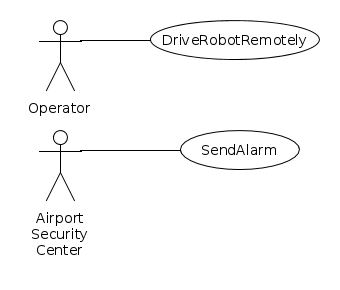
\includegraphics[scale=0.5]{./img/usecase.png}

\subsection{Scenarios}
\labelssec{Scenarios}
Scenario 1:\\ \\
\begin{tabular}{| l | l |}
	\hline
	\textbf{Title} & DriveRobotRemotely
	\\ \hline
	\textbf{Description}  & The operator drives the robot to the suspicious bag
	\\ \hline
	\textbf{Relationships} & 
	\\ \hline
	\textbf{Actors} & Operator
	\\ \hline
	\textbf{Preconditions} & The robot is in the RBA, waiting for commands from the operator.
	\\ \hline
	\textbf{Postconditions} & The robot starts the detection phase.
	\\ \hline
	\textbf{Main scenario} & The operator uses the remote console to drive the robot. \\ &
	When the robot perceives the bag, it starts the detection phase.
	\\ \hline
\end{tabular}
\\ Scenario 2:\\ \\
\begin{tabular}{| l | l |}
	\hline
	\textbf{Title} & SendAlarm
	\\ \hline
	\textbf{Description}  & The Airport Security Center sends an alarm signal to the robot if \\ & needed
	\\ \hline
	\textbf{Relationships} & 
	\\ \hline
	\textbf{Actors} & Airport Security Center
	\\ \hline
	\textbf{Preconditions} & The Airport Security Center received the detection results
	\\ \hline
	\textbf{Postconditions} & The robot blinks its led until it comes back to the RBA.
	\\ \hline
	\textbf{Main scenario} & 
	The Airport Security Center uses its interface to send the alarm \\ & to the robot.
	The robot blinks its led.
	\\ \hline
\end{tabular}

%\subsection{Requirements model}
%\labelssec{Requirements model}
\newpage
\subsection{(Domain) model}
\labelssec{Domain model}
In this phase we try to find an agreement with the client on what the entities mentioned in the requirements are and what they have to do.\\The system is composed by three parts:
\begin{itemize}
\item \textbf{Operator's remote console}
\item \textbf{Airport Security Center's remote console}
\item \textbf{Differential drive robot}
\end{itemize}
A \textbf{console} is a physical or virtual device that allows communication between the system and an external entity. It can get user input data and send them to the system, show some system output data to the user or both. In this case, the operator's console can get input from the operator and the Airport Security Center's console can receive the detection results and emit an alarm signal.
\\A \textbf{differential drive robot} is a composed entity that is able to use some devices to perform actions and receive data from the environment. It can also communicate with other parts of the system. All differential drive robots must have a sonar and are able to move in the environment. In this case, the differential drive robot has DC motors and wheels to move, a sonar, a led and a camera.
DC motors, wheels, led, sonar and camera are the hardware components mounted on the robot.
\\A \textbf{DC motor} can spin the attached wheel clockwise or counter-clockwise.
\\A \textbf{led} can be turned on or off.
\\A \textbf{sonar} can send an ultrasonic signal (trigger) and generates a corresponding response waveform (echo). The waveform analysis allows to estimate the distance from an obstacle.
\\ A \textbf{camera} is a device that can take photos when requested. It will be used by the robot in the detection phase.\\ \\
We want to define the system formally so that we can avoid ambiguity and generate an executable version of said model, but we want to avoid any technology assumption. To achieve this, we will use the custom language / executable meta-model developed by our software house. It allows us to describe what the parts of the system are, how they interact with each other and their behaviour and it can generate the corresponding executable code.\\ \\
The following is a first description of the system obtained by the requirement analysis:
%inserire qui il listato .ddr di analisi dei requisiti
\lstinputlisting[language=ddr, frame=single]{../TestCase2016Analysis/src/it/unibo/sartiballanti/testcase2016/analysis/analysis.ddr}
The operator can only send commands to drive the robot.
The Airport Security Center waits for the detection results and can emit the alarm only after the results have been sent.
%\subsection{System model}
\newpage
\subsection{Test plan}
We can do a test plan even before starting to implement the application, as a way to specify the expected behaviour of the system in a precise way. We just need to check if the parts of the system behave and interact with each other as defined in the requirements.
We can't express tests formally tough, because we already described the entities as actors, so object oriented tests (e.g. JUnit tests) are inadequate. Furthermore, some tests should check the interaction of the physiscal system with the environment and this can only be achieved by observing the actual behaviour of the system. Thus, we'll describe these tests in natural language.\\
In the initial phase, the operator drives the robot. We have to check the following:
\begin{itemize}
\item the operator can send commands to the robot
\item the robot executes the commands it receives
\item the robot accepts commands only from a single source
\item the robot perceives the presence of an obstacle
\end{itemize}
In the detection phase, the robot inspects the bag. We'll test the following:
\begin{itemize}
\item the robot stops and ignores commands from the operator
\item the robot starts blinking after it stopped
\item the robot can take a picture of the bag
\item the robot can send the results to the Airport Security Center
\item the Airport Security Center can receive the results of the inspection
\item the robot stops blinking at the end of this phase
\end{itemize}
In the final phase, the robot comes back to the RBA. These are the tests we'll do:
\begin{itemize}
\item the robot actually comes back autonomously
\item the Airport Security Center can emit the alarm signal
\item the robot blinks the led if it perceives the alarm
\end{itemize}
At this stage in the development process, we can't define more specific functional or integration tests, we'll add them as needed during the implementation phase.
We still haven't decided what technology we will use to implement the application, so we can't write executable tests yet. However, at the end of the analysis phase, we'll have an executable logical architecture of the application and we'll be able to perform some of the tests on it.
\newpage
%===========================================================================
\section{Problem analysis}
\labelsec{ProblemAnalysis}
%===========================================================================
\subsection{Logic architecture}
Logic architecture can be expressed in 3 dimensions:
\begin{enumerate}
\item \textbf{Structure}: what parts the system is made of.
\item \textbf{Interaction}: how the parts of the system communicate with each other.
\item \textbf{Behaviour}: what the parts of the system do.
\end{enumerate}
We can formally express these concepts with the DDR custom language:
\lstinputlisting[language=ddr, frame=single]{../TestCase2016LogicArchitecture/src/it/unibo/sartiballanti/testcase2016/analysis/logicArchitecture.ddr}
This describes the whole logic architecture of our application. It can also be executed so that the client can confirm that the analysis defined a system that behaves as required.\\
This architecture derives from the one obtained in the domain model and introduces new interactions and a new entity.\\
The \textbf{DriveRobot} receives commands from the Operator Interface in the first phase, executes its automatic operations during the detection phase, it sends results to the ASCConsole and comes back to the RBA in the end. It has to react to obstacles to begin the detection phase.\\
The \textbf{Operator Console} receives commands from the operator as events and sends the corresponding commands to the robot.\\
The \textbf{ASC Console} receives the detection results from the detection phase and then enables the Airport Security Center to emit the alarm.\\
We decided to introduce the \textbf{led} as an actor separated from the robot because it is an active entity that has to sense and react to system events and has its own behaviour, so modeling it as a passive object managed by the robot is inappropriate. The led starts to blink when the detection phase begins, stops to blink when the detection phase ends and it starts to blink again if the alarm is emitted when the robot is coming back. Finally it stops blinking when the robot reaches the RBA.\\
The \textbf{camera} will be modeled as a passive entity that can only take a picture when the robot asks for it.\\
We defined the accessory event botIsBack to signal that the robot has come back to the RBA. This event can be used to stop the led if an alarm has been emitted before.\\
The interaction with external entities (the operator and the ASC) have been modeled as local events.
\subsection{Abstraction gap}
The abstraction gap is the distance between the concepts used to model the problem and those implied by the technology available.
Based on the previous analysis, we found out that this application needs a set of features that includes:
\begin{itemize}
\item Synchronous and asynchronous communication between heterogeneous parts of a distributed system
\item Distributed events
\item Communication with entities that are not part of the system
\item Interruptable actions
\end{itemize}
All the features we need can be implemented with current technology: actually, the framework developed by our software house can offer these features.
\subsection{Risk analysis}
Thanks to the framework provided, executable code is generated from the model defined in the ddr meta-model. Thus, adopting this framework allows the application designers to use an extremely high-level description of the problem, closer to the application domain, reducing considerably the abstraction gap. The specific technology to be used can be decided later, during implementation phase. The advantage of using a meta-model and a code generator is also that it can be extended to support more advanced concepts.
Using the framework code generators, we can write most of the code independently from the specific implementation technology. Although the qa/ddr metamodel is technology independent, the code generated automatically may require some kind of environment on the computational nodes where it will be deployed (e.g. the JVM, the .NET runtime environment, a specific operating system etc).
%===========================================================================
\section{Work plan}
\labelsec{wplan}
%===========================================================================
After the analysis phase, we decided to develop the application using the ddr framework, so that we don't start from scratch. We can reuse the executable logic architecture and enhance it. The framework already offers the implementation logic for some parts of the system and it offers high level abstractions that allow the developers to focus on business logic and not to worry too much about boilerplate code.\\
We'll use the following features offered by the framework:
\begin{itemize}
\item A communication system that allows the parts of the system to send and receive messages and events
\item Reactive actions
\item Timed actions
\item The robot configuration
\item DC motors driver
\item sonar driver (and management of its data)
\end{itemize}
We'll implement the remaining features following the SCRUM framework for work planning. So we defined a product backlog which is a prioritized list of tasks needed to complete the project:
\begin{enumerate}
\item Define the robot configuration with .baseddr
\item Implement the console interfaces that allow external entities to interact with the system
\item Implement the led driver
\item Decide and implement a way to send a picture in the ddr framework
\item Develop the detection phase logic with the camera driver (as a mock entity)
\item Create an algorithm that allows the robot to come back to the RBA
\end{enumerate}

%===========================================================================
\section{Project}
\labelsec{Project}
%===========================================================================
\subsection{Structure}
The structure is essentially the same as the logic architecture. Our robot has no camera, so we'll implement it as a mock device.
\subsection{Interaction}
There are no significant changes from the logic architecture.
\subsection{Behavior}
More details have been added to implement the missing features described in the work plan.\\
The consoles used by the ASC and the operator will be GUIs that allow them to interact with the system.
The robot behaviour has slightly changed in the first phase: to ensure it receives messages from a single source, it memorizes the sender of the first received drive message and accepts new drive commands from that source only.
\lstinputlisting[language=ddr, frame=single]{../TestCase2016Project/src/it/unibo/sartiballanti/testcase2016/project/project.ddr}
\newpage
%===========================================================================
\section{Implementation}
\labelsec{Implementation}
\subsection{Robot configuration}
The file robots.baseddr contains the configuration we used:
\lstinputlisting[firstline=7,lastline=16, frame=single]{../TestCase2016Project/src/it/unibo/sartiballanti/testcase2016/project/robots.baseddr}
\subsection{Operator and ASC console}
The \textbf{operator console} includes a GUI that translates external input events into messages to drive the robot.
\lstinputlisting[language=java, frame=single]{../TestCase2016Project/src/it/unibo/operatorconsole/Operatorconsole.java}
The \textbf{ASC console} includes a GUI that shows the image received from the robot at the end of the detection phase and then shows a button that emits the alarm if pressed.
\lstinputlisting[language=java, frame=single]{../TestCase2016Project/src/it/unibo/ascconsole/Ascconsole.java}
\subsection{Led}
The \textbf{led} blinking logic is implemented directly as QActor behaviour.\\
The Prolog theory turnTheLed/1 allows the QActor to manage the led and actually turn it on and off calling the underlying Java code.
\lstinputlisting[language=prolog, frame=single]{../TestCase2016Project/src/it/unibo/led/ledTheory.pl}
The led instance is created through a factory:
\lstinputlisting[language=java, frame=single]{../TestCase2016Project/src/it/unibo/devices/qa/LedDevicesFactory.java}
We implemented the led as a bash script that receives zeros and ones to turn the led on and off:
\lstinputlisting[language=java, frame=single]{../TestCase2016Project/src/it/unibo/devices/qa/LedShellCmdInterpreter.java}
\lstinputlisting[language=bash, frame=single]{../TestCase2016Project/bash/gpioPinInterpreter.sh}
\subsection{Camera}
The camera implements the following interface:
\lstinputlisting[language=java, frame=single]{../TestCase2016Project/src/it/unibo/sartiballanti/camera/ICamera.java}
This is the implementation of the mock camera:
\lstinputlisting[language=java, frame=single]{../TestCase2016Project/src/it/unibo/sartiballanti/camera/MockFileCamera.java}
\subsection{Detection phase}
The \textbf{robot} uses an actor method to execute the detection phase. It takes a picture of the bag using the simulated \textbf{camera} and sends it to the ASC. In order to send send the photo as a message payload in the ddr framework, we needed to obtain a string representation of the image.\\
\lstinputlisting[language=java, frame=single]{../TestCase2016Project/src/it/unibo/driverobot/Driverobot.java}
\subsection{Back to base}
The \textbf{driveRobotTheory} is used to implement a simple algorithm to come back autonomously: the robot memorizes every move it makes in the first phase, so it can come back executing the same moves backwards.\\
\lstinputlisting[language=prolog, frame=single]{../TestCase2016Project/src/it/unibo/driverobot/driveRobotTheory.pl}
\newpage
%===========================================================================
\section{Testing}
\labelsec{testing}
%===========================================================================
In the previous sections, we had an executable model that could be tested, so most of the tests that involve communication between parts of the system have been done at the end of the analysis phase. Initially, communication tests have been executed locally, then the system parts have been deployed on different computational nodes to test system behaviour as a whole in a distributed environment, checking if the system behaved as described in the test plan.
In local tests, we used a mock robot that simulated sensors and motors:
\lstinputlisting[firstline=22,lastline=33,frame=single]{../TestCase2016Project/src/it/unibo/sartiballanti/testcase2016/project/robots.baseddr}
Finally, we deployed the system parts on their final location and tested the complete system and checked that it behaved as described in the test plan.
%===========================================================================
\section{Deployment}
\labelsec{Deployment}
%===========================================================================
The parts of the application will be deployed on different computational nodes as JAR executable archives with some configuration files, Prolog theories and bash scripts.
The platforms we use in this case are a Raspberry Pi board on the robot and two PCs to provide the consoles, we just need to copy the appropriate files, set execution permissions for the bash scripts and execute the JAR on every node. The application will start when all the parts of the system have been started.
%===========================================================================
\section{Maintenance}
\labelsec{Maintenance}
We developed the application using the ddr framework and delaying any technological hypothesis, so the resulting system can be easily modified to add or change features. In the next section, we'll show how new (compatible) requirements need very little changes to the previously developed system.
%===========================================================================
\section{Step 2}
\subsection{Requirements}
\textbf{STEP 2 (Implementation Optional)}\\
Extend the last requirement as follows:
\begin{itemize}
\item If the bag is qualifed as "harmful", the Airport Security Center emits an 'alarm' signal and activates another (properly equipped) robot that (starting from the same RBA of the robot inspector) should reach the bag in autonomous way and remove the bag from the area.
\end{itemize}
\subsection{Requirements analysis}
\subsubsection{Use cases}
No new use cases or changes to the previous ones.
\subsubsection{Scenarios}
No new scenarios or changes to the previous ones.
\subsubsection{(Domain) model}
A new robot is introduced, similar to the previous one. It needs a way to remove the bag. We just need to add the following to the previous domain model:
\lstinputlisting[language=ddr, frame=single]{../TestCase2016ExtensionAnalysis/src/it/unibo/sartiballanti/testcase2016/extension/analysis/analysis.ddr}
\subsubsection{Test plan}
We need to check if the second robot receives can reach the bag and remove it. We can test this observing the whole system after the ASC emits the alarm.
\subsection{Problem analysis}
\subsubsection{Logic architecture}
We can obtain the new logic architecture adding a new type of message, the new actor described in the domain model and slightly changing the behavior of the first robot.\\
It is not specified by the requirements whether the second robot has to go to the bag as soon as it perceives the alarm, or it can wait until the first robot is returned to the RBA. If it has to start immediatly, collisions may occur during the route. So, in order to avoid this problem, we'll make the second robot wait for the first one. In any case, the second robot should know the bag location as soon as possible. Thus, the first robot will send the route to the bag to the second robot immidiately after it reached the bag. The second robot will follow this route to reach the bag and remove it if an alarm is emitted.
\lstinputlisting[language=ddr, frame=single]{../TestCase2016ExtensionLogicArchitecture/src/it/unibo/sartiballanti/testcase2016/extension/analysis/logicArchitecture.ddr}
\subsection{Work plan}
We are using the ddr framework, so most of the behaviour of the new robot is already defined. The bag removal will be simulated with a print operation because our robot can't physically move the bag, so we just need to define the second robot configuration and implement an algorithm that allows the robot to follow the route it received from the other robot. 
\subsection{Project}
\subsubsection{Structure}
The structure is the same as the logic architecture.
\subsubsection{Interaction}
We introduced the message routeToBag to send the path to follow to the second robot. 
\subsubsection{Behavior}
The behavior of the asc console, operator console and led remain unchanged, the first robot just needs to send a new message as described before. The second robot has no actuators, so it will just simulate the bag removal.
\lstinputlisting[language=ddr, frame=single]{../TestCase2016ExtensionProject/src/it/unibo/sartiballanti/testcase2016/project/project.ddr}
\subsection{Implementation}
This is the configuration of the new robot:
\lstinputlisting[firstline=32,lastline=41,frame=single]{../TestCase2016ExtensionProject/src/it/unibo/sartiballanti/testcase2016/project/robots.baseddr}
We use the following Prolog theory to make the robot reach the bag:
\lstinputlisting[language=prolog, frame=single]{../TestCase2016ExtensionProject/src/it/unibo/removerobot/removeRobotTheory.pl}
The bag removal is just a print operation done by the actor.
\subsection{Testing}
We tested the system as a whole observing the second robot when an alarm is emitted.


\newpage
See \cite{natMol09} until page 11 (\texttt{CMM}) and pages 96-105.

%===========================================================================
\section{Information about the author}
\labelsec{Author}
%===========================================================================

\vskip.5cm
%%% \begin{figure}
\begin{tabular}{ | c |  }
\hline
  % after \\: \hline or \cline{col1-col2} \cline{col3-col4} ...
  Paolo Sarti 
  \\
   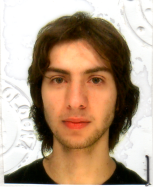
\includegraphics[scale = 0.7]{img/author_scaled.png}
  \\
\hline
\end{tabular}
\begin{tabular}{ | c |  }
\hline
  % after \\: \hline or \cline{col1-col2} \cline{col3-col4} ...
  Marcello Ballanti 
  \\

   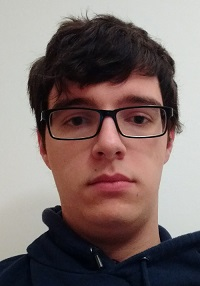
\includegraphics[scale = 0.35]{img/io2.jpg}
  \\
\hline
\end{tabular}


%%% \begin{itemize}
%%% \item Titolo di studio:\\ \\
%%% \item Interessi particolari:\\ \\
%%% \item Ha sostenuto fino ad oggi il seguente numero di esami:\\ \\
%%% \item Deve ancora sostenere i seguenti esami del I anno:\\ \\
%%% \item Prevede di svolgere un tirocinio presso:\\ \\
%%% \item Prevede di laurearsi nella sessione:\\ \\
%%% \item Intende proseguire gli studi per conseguire: \\  \\  \\
%%%   	presso la sede universitaria di: \\ \\
%%% \item Intende entrare subito nel mondo del lavoro presso : \\ \\
%%% \end{itemize}

 
\appendix


\bibliographystyle{abbrv}
\bibliography{biblio}

\end{document}












